\documentclass[letterpaper,12pt]{article}

\usepackage[margin=1.0in]{geometry}
\usepackage{multirow}
\usepackage{tikz}
\usepackage{amsmath}

\usetikzlibrary{shapes.geometric, arrows, fit}

\newcommand{\botname}{\textit{The Gans Cannon}}
\newcommand{\specialcell}[2][c]{\begin{tabular}[#1]{@{}c@{}}#2\end{tabular}}
\newcommand{\xxx}[1]{{\color{red}\bf #1}}
\newcommand{\AxisRotator}[1][rotate=0]{\tikz [x=0.25cm,y=0.60cm,line width=.2ex,-stealth,#1] \draw (0,0) arc (-150:150:1 and 1);}

\begin{document}

\title{T-Shirt Cannon Software Architecture}
\author{Hazen Eckert \hspace{3mm} Omar Hasan \hspace{3mm} Ryan Marcotte \hspace{3mm} Ridhwaan Rahman}
\date{}
\maketitle

\section{System Overview}

\begin{figure}[h!]
  \centering

  \tikzstyle{block} = [rectangle, rounded corners, minimum width=3cm, minimum height=2cm,text centered, draw=black]
  \tikzstyle{container} = [draw, rectangle, rounded corners, dashed, text width=11em, inner sep=3.5em]
  \tikzstyle{arrow} = [thick, ->, >=latex]
  \begin{tikzpicture}[node distance=2cm]
    \node (input) [align=center, xshift=-1cm] {User\\Inputs};
    \node (output) [right of=input, align=center] {Video\\Display};
    \node (computer) [block, yshift=-2cm] {Computer};
    \node (ar9331) [block, right of=computer, xshift=9cm, yshift=-2cm, align=center] {Atheros\\AR9331};
    \node (atmega) [block, below of=ar9331, yshift=-2cm, align=center] {Arduino\\ATmega32u4};
    \node (rpi) [block, right of=computer, above of=ar9331, xshift=-2cm, yshift=2cm] {Raspberry Pi};

    \node (yun) [container, fit=(atmega) (ar9331)] {};
    \node (yun_text) [yshift=-0.3cm] at (yun.north) {Yun};

    \draw [arrow] (computer.336) -- node[anchor=east, align=center, yshift=-5mm] {Velocity\\Commands} (ar9331.188);
    \draw [arrow] (ar9331.172) -- node[anchor=west, align=center, xshift=-12mm, yshift=5mm] {Status Updates} (computer.352);
    \draw [arrow] (ar9331.240) -- node[anchor=east, align=center] {GPIO\\Commands} (atmega.120);
    \draw [arrow] (atmega.60) -- node[anchor=west, align=center] {Sensor\\Readings} (ar9331.300);
    \draw [arrow] (rpi.172) -- node[anchor=east, align=center, yshift=5mm] {Video\\Stream} (computer.24);
    \draw [arrow] (computer.8) -- node[anchor=west, align=center, xshift=-12mm, yshift=-5mm] {Video Commands} (rpi.188);
    \draw [arrow] (input) -- (computer.134);
    \draw [arrow] (computer.46) -- (output);
  \end{tikzpicture}
  \caption{System Overview}
  \label{fig:system_diagram}
\end{figure}

\subsection{Computer}
\subsection{AR9331}
\subsubsection{Velocity Kinematics}

\noindent In order to command a desired robot velocity,
\begin{math}
  v=
  \begin{bmatrix}
    v_x \\
    v_y \\
    \omega_z
  \end{bmatrix}
\end{math}
, we calculate the wheel velocities as shown in Equations \ref{eq:rw_to_v}-\ref{eq:v_wheel_4}, according to Figure \ref{fig:robot_top_view}.

\begin{figure}[h!]
  \centering

  \tikzstyle{robot} = [rectangle, minimum width=3cm, minimum height=4cm,text centered, draw=black]
  \tikzstyle{wheel} = [rectangle, minimum width=5mm, minimum height=1cm, draw=black]
  \tikzstyle{arrow} = [thick, ->, >=latex]
  \tikzstyle{dist} = [thick, <->, >=|]

  \begin{tikzpicture}
    \node (robot) [robot] {};
    \node (wheel 1) [wheel, left of=robot, xshift=-7.5mm, yshift=1cm] {1};
    \node (wheel 2) [wheel, right of=robot, xshift=7.5mm, yshift=1cm] {2};
    \node (wheel 3) [wheel, right of=robot, xshift=7.5mm, yshift=-1cm] {3};
    \node (wheel 4) [wheel, left of=robot, xshift=-7.5mm, yshift=-1cm] {4};

    \draw [arrow] (0,0) -- node[anchor=north, xshift=-4mm] {y} (-1,0);
    \draw [arrow] (0,0) -- node[anchor=west, yshift=5mm] {x} (0,1);
    \draw (0,0)  -- (0,0) node[xshift=2.8mm] {\AxisRotator[x=0.3cm,y=0.3cm,->,rotate=-90,black] $\omega_z$};
    \draw [dist] (0,2.3) -- node[anchor=south] {$l_1$} (1.8,2.3);
    \draw [dist] (0.03,2.3) -- node[anchor=south] {$l_1$} (-1.8,2.3);
    \draw [dist] (0,-2.3) -- node[anchor=north] {$l_1$} (1.8,-2.3);
    \draw [dist] (0.03,-2.3) -- node[anchor=north] {$l_1$} (-1.8,-2.3);
    \draw [dist] (2.3,0) -- node[anchor=west] {$l_2$} (2.3, 1);
    \draw [dist] (2.3,0.03) -- node[anchor=west] {$l_2$} (2.3, -1);
    \draw [dist] (-2.3,0) -- node[anchor=east] {$l_2$} (-2.3, 1);
    \draw [dist] (-2.3,0.03) -- node[anchor=east] {$l_2$} (-2.3, -1);
  \end{tikzpicture}
  \caption{Top View of Robot}
  \label{fig:robot_top_view}
\end{figure}

\begin{equation}
  v_{wheel}=r_{wheel}\omega_{wheel}
  \label{eq:rw_to_v}
\end{equation}
\begin{equation}
  v_{wheel\,1}=v_x-v_y-(l_1+l_2)\omega_z
  \label{eq:v_wheel_1}
\end{equation}
\begin{equation}
  v_{wheel\,2}=v_x+v_y+(l_1+l_2)\omega_z
  \label{eq:v_wheel_2}
\end{equation}
\begin{equation}
  v_{wheel\,3}=v_x+v_y-(l_1+l_2)\omega_z
  \label{eq:v_wheel_3}
\end{equation}
\begin{equation}
  v_{wheel\,4}=v_x-v_y+(l_1+l_2)\omega_z
  \label{eq:v_wheel_4}
\end{equation}


\subsection{ATmega32u4}
\subsection{Raspberry Pi}

\section{Application Interface Specifications}

\subsection{Message Formats}

\subsubsection{Origin: Computer}

\xxx{Describe the formats of each message type that will be sent from the computer to the robot. The first byte of each message will identify its type and tell how to interpret the rest of the message. If we are going to be using a Pi in addition to the Yun, some message types will actually be addressed to the Yun and others will be addressed to the Pi}

\begin{table}[h!]
  \centering
  \begin{tabular}{| c | c |}
    \hline
    \textbf{Field} & 0 \\
    \hline
    \textbf{Description} & \specialcell{Command\\Type} \\
    \hline
    \textbf{Value} & 0 \\
    \hline
  \end{tabular}
  \caption{Query Command Message Format}
  \label{tab:query_cmd_msg}
\end{table}

\begin{table}[h!]
  \centering
  \begin{tabular}{| c | c | c | c | c |}
    \hline
    \textbf{Field} & 0 & 1 & 2 & 3 \\
    \hline
    \textbf{Description} & \specialcell{Command\\Type} & \specialcell{Linear\\Velocity\\X} & \specialcell{Linear\\Velocity\\Y} & \specialcell{Angular\\Velocity} \\
    \hline
    \textbf{Value} & 1 & -128 to 127 & -128 to 127 & -128 to 127 \\
    \hline
  \end{tabular}
  \caption{Velocity Command Message Format}
  \label{tab:vel_cmd_msg}
\end{table}

\begin{table}[h!]
  \centering
  \begin{tabular}{| c | c |}
    \hline
    \textbf{Field} & 0 \\
    \hline
    \textbf{Description} & \specialcell{Command\\Type} \\
    \hline
    \textbf{Value} & 2 \\
    \hline
  \end{tabular}
  \caption{Fire Command Message Format}
  \label{tab:fire_cmd_msg}
\end{table}

\subsubsection{Origin: AR9331}

\subsubsection{Origin: Raspberry Pi}

\section{Chassis}
\begin{center}
    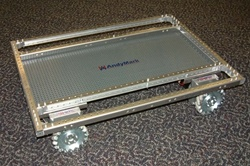
\includegraphics[width=11cm]{pics/chassis/andymark_chassis.jpg}
\end{center}

\subsection{Overview}
\botname's Chassis is the AndyMark C-Chassis with Mecanum Wheel Drive. This chassis was chosen among others because of its price, modularity, and size.

\subsection{Assembly}
\subsection{Troubleshooting}
\subsection{References}

\begin{table}[h!]
  \begin{tabular}{| c | c |}
    \hline
    \textbf{AndyMark Frame Assembly} &  http://files.andymark.com/am-0952AssemblyInstructions.pdf\\
    \hline
    \textbf{AndyMark Gearbox Assembly} &  http://files.andymark.com/x2010-toughbox-user-guide.pdf\\
    \hline
  \end{tabular}
  \label{tab:fire_cmd_msg}
\end{table}

\section{T-Shirt Cannon}
\begin{center}
    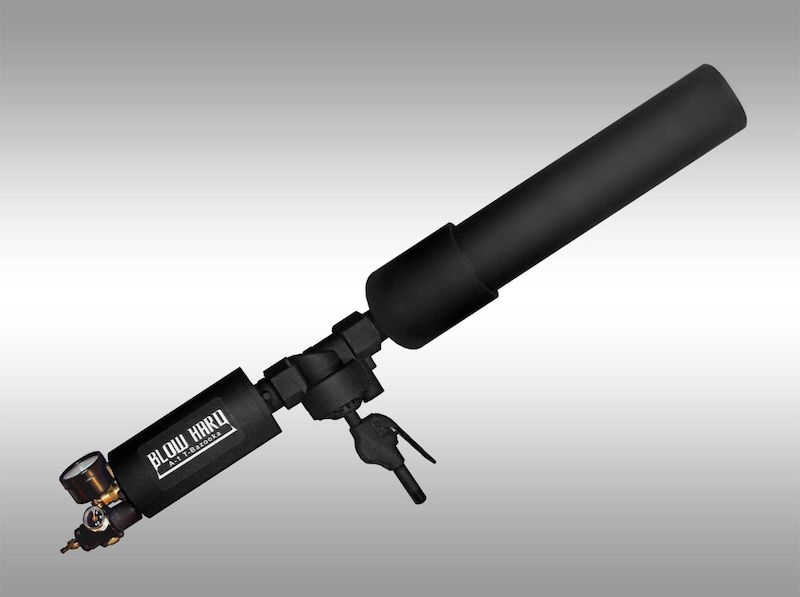
\includegraphics[width=11cm]{pics/cannon/blowhard_cannon.jpg}
\end{center}

\subsection{Troubleshooting}
\begin{center}
    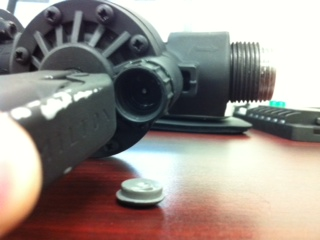
\includegraphics[width=11cm]{pics/cannon/broken_release_valve.jpg}
\end{center}


\end{document}
